\documentclass[parskip=full]{scrartcl}
\usepackage[utf8]{inputenc} % use utf8 file encoding for TeX sources
\usepackage[T1]{fontenc}    % avoid garbled Unicode text in pdf
\usepackage[german, english]{babel}  % german hyphenation, quotes, etc
\usepackage{graphicx}       % provides commands for including figures
\usepackage{rotating}
\usepackage{amsmath}
\usepackage{pdfpages}
\graphicspath{ {images/} }
\usepackage{hyperref}       % detailed hyperlink/pdf configuration
\hypersetup{                % ‘texdoc hyperref‘ for options
pdftitle={PSE : LAMeetsML},%
bookmarks=true,%
}
\usepackage{csquotes}       % provides \enquote{} macro for "quotes"
\usepackage[nonumberlist, acronym]{glossaries} % provides glossary commands
\usepackage{enumitem}
\usepackage{lscape}
\usepackage{caption}
%\usepackage{placeins}
\usepackage[section]{placeins}

%\documentclass[12pt, oneside]{book}
\usepackage{wrapfig}
\usepackage{epstopdf}
\usepackage{caption, subcaption}



\makenoidxglossaries
%
%%Glossary
%

\begin{document}

\begin{titlepage}
\centering
{\scshape\LARGE Karlsruher Institut für Technologie\par}
\vspace{1cm}
{\scshape\Large Test Report Document \par}
\vspace{1.5cm}
{\huge\bfseries Numerical Linear Algebra meets Machine Learning \par}
\vspace {2cm}

{\Large\itshape Fabian Koffer\par}
{\Large\itshape Simon Hanselmann\par}
{\Large\itshape Yannick Funk\par}
{\Large\itshape Dennis Leon Gr\"{o}tzinger\par}
{\Large\itshape Anna Katharina Ricker\par}

\vfill
Supervisors\par
Hartwig Anzt
Markus G\"{o}tz


\vfill
{\large\today\par}
\end{titlepage}

\tableofcontents
\newpage

\section{Stats}

Lines of Code:

Python:
C++:

others:

Test Coverage:	

\newpage

\section{Continuous Integration}

To ensure a high quality on our code, we increased the building process of our code.

%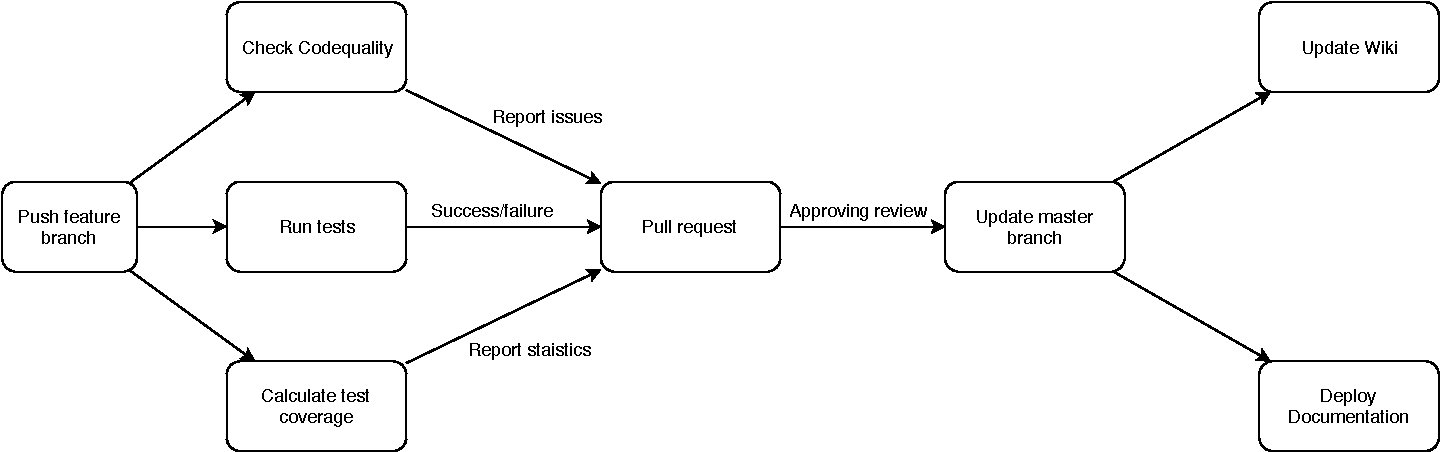
\includepdf[width=\textwidth, keepaspectratio]{build_process.pdf} bad ratio

When pushing a branch, not just the test are ran on Travis, but also we generate a coverage report that will be sent to CodeClimate.
This way you get a small overview on each pull request about the current coverage and the coverage on the newly committed lines.
Added to that, you can get a complete overview on the
\href{https://codeclimate.com/github/TheSlimvReal/PSE---LA-meets-ML}{CodeClimate Webpage}.

After a successful merge to the master, we also introduced two new deployment steps.
The first is that the wiki pages on GitHub are build again in case a change happened on this files.
The second step is that we generate a code documentation is generated and uploaded to GitHub pages.

\newpage

\section{Code Documentation}

In the first phases we already decided to comment our code with the Doxygen-Syntax.
In the implementation phase we took good care in documenting our code properly.
The problem now was that everyone would have to generate this documentation for himself, which is a lot of work.

To easy things up, we added a deployment step, which generates this documentation and deploys it to GitHub pages.

This way everybody can have a look at the latest version of the documentation only be opening a link.

\newpage

\section{Wiki}

We already collected some documentations for working with our project in the previous phases and decided to make them available in the GitHub wiki.
Because the GitHub wiki holds its own git structure and we wanted to keep all our files in one place, we decided to integrate the wiki in our build process.

Therefore we created a folder in the projects root which holds all the wiki's entries in markdown files together with an configuration file.
This configuration file is used to dynamically generate a sidebar that holds a navigation for the wiki entries.
All the contents of this folder together with the generated sidebar are then copied to the wiki's git.

After this is done, the new wiki entries can be found on GitHub.

\newpage

\section{Bugs}
\begin{tabular}{|p{4.5cm}|p{4.5cm}|p{2cm}|p{1.5cm}|}

\hline

 Description  & Fix & Time to Fix & Reporter  \\

\hline

Command line input with more than one space between arguments resulted in program crash & 
Changed the parameters of the string-split function for the expected behavior (remove spaces) &
2 hours &
Anna \\

\hline

Corrupted configuration file results in a program crash &
Opening config file now happens in a try-except block and errors are reported to user (no crash) &
1.5 hours &
Simon \\

\hline

Labeling or collection on operating systems other than linux resulted in crashes &
Current OS is checked at start of module and wrong OS's are reported to user &
2 hours &
Simon\\

\hline

User entered size parameter was not used in collector &
Removed static size declaration and started using the size input parameter &
1 hour &
Anna \\

\hline

Default parameters are not correctly passed to the modules &
Config file had wrong format, needed to be fixed/standardized &
3 hours &
Simon \\

\hline
\end{tabular}

\newpage
\section{Glossary}
%\glspl{collector}, labeling modle, neural network, classifier, default settings  \glspl{Dateiformat}

% % Automatisch generiertes Glossar (Latex zwei mal ausführen um Glossar anzuzeigen)
%
%\glsaddall % das sorgt dafür, dass alles Glossareinträge gedruckt werden, nicht nur die verwendeten. Das sollte nicht nötig sein!
\printnoidxglossaries

\end{document}

